%!TeX encoding=utf8
\documentclass[ngerman]{scrartcl} 

% Passen Sie hier *Author1*, *Author2* und *Grp.-Nr.* an.
\newcommand{\authA}{Alexander Steding}

\newcommand{\grpnr}{4}
\usepackage{array}
\usepackage{longtable}

% Optionen für die Dokumentenklasse scartcl von KOMAscript. 
\KOMAoptions{
	DIV=11,
	BCOR=0mm,
	paper=a4,
	fontsize=12pt,
	parskip=half,
	twoside=false,
	titlepage=false
}
\usepackage{booktabs}

% Papierformat: DIN-A4, mit wenig Rand 
\usepackage[
	a4paper,
	left=20mm,
	right=20mm,
	top=23mm, 
	bottom=18mm,
	includefoot,
	footskip=8mm
	]{geometry}

% Zeilenabstand, andere Werte: onehalfspacing, doublespacing
\usepackage[singlespacing]{setspace} 

% Definition der Kopf- und Fußzeile
\usepackage[headsepline,automark]{scrlayer-scrpage}
\clearscrheadings
\setlength{\headheight}{2.5\baselineskip}
\setlength{\footheight}{1\baselineskip}
\chead[]{ \\  Abschlussbericht}
\ihead[]{\\ \authA}
\ohead[]{Datum: \today }
\ofoot[]{\pagemark}

%---Language and umlauts
\usepackage[utf8]{inputenc}       % UTF-8 Kodierung - ä, ö, ü, ß direkt eingeben
\usepackage[ngerman]{babel}                      % Neue deutsche Rechtschreibung  
\usepackage[expansion=true, protrusion=true]{microtype} % Bessere Silbentrennung

% Formelsatz
\usepackage{amsmath}		% Mathematik-Umgebungen - z.B. align
\usepackage{amsthm}		% Umgebung "theorem"
\usepackage{amsfonts}	% Schriften
\usepackage{amssymb}		% Symbole
\usepackage{upgreek}		% Griechische Sonderzeichen z.B. \upmu
\usepackage{booktabs}
% Einheiten
\usepackage{siunitx}
\sisetup{
	locale = DE,  
	separate-uncertainty,  
	range-units = brackets,  
	list-units = single,  
	per-mode=fraction
}

% Bilder und Tabellen
\usepackage{graphicx}			% Bilder als PDF einbinden
\usepackage{epstopdf}			% Bilder im EPS-Format
\usepackage{caption}				% Unterschriften für Bilder und Tapellen
\usepackage{booktabs}			% Zusätzliche Schönheitslinien für Tabellen
\usepackage{multirow}			% Mehrere Felder in einer Tabelle zusammenfassen
\usepackage[table]{xcolor}		% Für farbig unterlegte Tabellenzeilen
  \definecolor{lightgray}{gray}{0.9}
  \rowcolors{1}{}{lightgray}	% jede zweite Zeile in einer Tabelle leicht grau


% Positionierung von Bildern und Tabellen
\usepackage{float}				% Option 'H', also "hier-egal-wie-das-aussieht"
\usepackage[section]{placeins}	% Platzierung spätestens am Ende eines Kapitels
\renewcommand{\floatpagefraction}{.75}	% standard: .5
\renewcommand{\textfraction}{.1}			% standard: .2
\renewcommand{\topfraction}{.8}			% standard: .7
\renewcommand{\bottomfraction}{.5}		% standard: .3
\setcounter{topnumber}{3}				% standard: 2
\setcounter{bottomnumber}{2}				% standard: 1
\setcounter{totalnumber}{5}				% standard: 3

\usepackage{caption}
\captionsetup[figure]{name=Abb.}
\captionsetup[table]{name=Tab.}

% Hyperlinks
\usepackage{hyperref}
\hypersetup{
	colorlinks=true, 
	breaklinks=true, 
	citecolor=darkgray, 
	linkcolor=darkgray, 
	menucolor=red, 
	urlcolor=cyan,
	bookmarksopen=false, 
	bookmarksopenlevel=0,
	plainpages=false,			% zur korrekten Erstellung der Bookmarks 
	hypertexnames=false			% zur korrekten Erstellung der Bookmarks 
}

\usepackage{pdfpages} 		% Einfügen von Vollseiten-PDFs (z.B. das Deckblatt)
\usepackage{csquotes}		% Zitate
\usepackage{pythonhighlight}
% Literaturverzeichnis
\usepackage[style=alphabetic,sorting=ynt,backend=biber]{biblatex}

% Eine Abkürzung, die Computerbefehle im Fließtext mit einer Mono-Schrift setzt
% (funktioniert leider nicht für Backslash \ . Da hilft dann der Befehl \verb )
\providecommand*{\code}[1]{{\texttt{#1}}}
\usepackage{listings}
\usepackage{xcolor}

\definecolor{codegreen}{rgb}{0,0.6,0}
\definecolor{codegray}{rgb}{0.5,0.5,0.5}
\definecolor{codepurple}{rgb}{0.58,0,0.82}
\definecolor{backcolour}{rgb}{0.95,0.95,0.92}

\lstdefinestyle{mystyle}{
    backgroundcolor=\color{backcolour},   
    commentstyle=\color{codegreen},
    keywordstyle=\color{magenta},
    numberstyle=\tiny\color{codegray},
    stringstyle=\color{codepurple},
    basicstyle=\ttfamily\footnotesize,
    breakatwhitespace=false,         
    breaklines=true,                 
    captionpos=b,                    
    keepspaces=true,                 
    numbers=left,                    
    numbersep=5pt,                  
    showspaces=false,                
    showstringspaces=false,
    showtabs=false,                  
    tabsize=2
}

\lstset{style=mystyle}
\usepackage{hyperref}
\begin{document}
\shorthandoff{"}           % Anführungszeichen nicht als Befehl interpretieren



\begin{titlepage}
\begin{center}
\vspace{3cm}
{\fontsize{40}{49} \selectfont \textbf{Programierpraktikum Übung 4}}\\[2cm]
\Large{\authA }\\
\Large{10028034 }\\
\large{Gottfried Wilhelm Leibniz Universität\\{\today}}
\end{center}
\end{titlepage}
\stepcounter{page}

\newpage
\tableofcontents
\newpage
\section{Einleitung }
Dieser Bericht stellt als Abschlussbericht die Ergebnisse und Erkenntnisse des Programmierpraktikums Schadstoffausbreitung zusammen. Als Programmiersprache wurde über alle Aufgaben hinweg Julia verwendet und als Graphisches Backend PlotlyJS.
\section{Aufgabe  1}
Ziel dieser Aufgabe ist es ein Gauß-Modell für eine kontinuierliche Linienquelle zu Programmieren und anschließend die Maximalkonzentration am Erdboden zu bestimmen.

In Aufgabenteil b wird ein Monte-Carlo-Modell für eine kontinuirliche Linienquelle programmiert und mit dem Gauß-Modell aus Aufgabenteil a verglichen.
\subsection{Aufgabenteil a}
In Abbildung 1. ist die zu erwartende Konzentrationsverteilung des Gauß-Modells als X-Z-Schnitt visualisiert.
\begin{figure}[H]
	\centering
	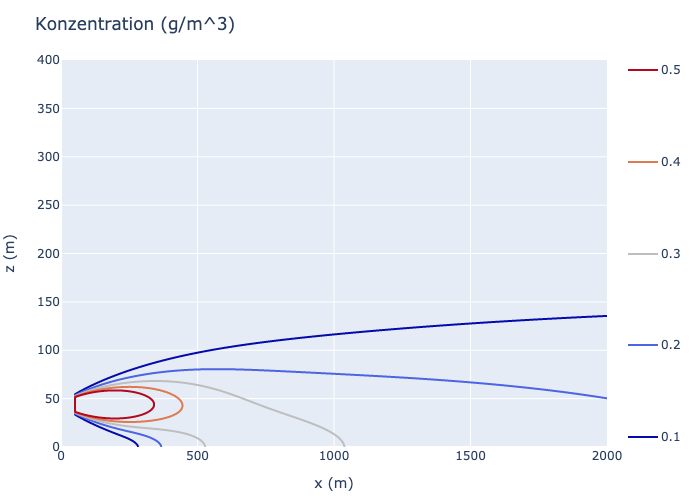
\includegraphics[scale=0.5]{Bilder/1a.png}
	\caption{Konzentrationsverteilung}
	\label{fig:my_label}
\end{figure}
Für eine feinere grapische Analyse wurde in Abbildung 2. die Konzentrationsverteilung am Erdboden, also für $z=\si{m}$, visualisiert.
\begin{figure}[H]
	\centering
	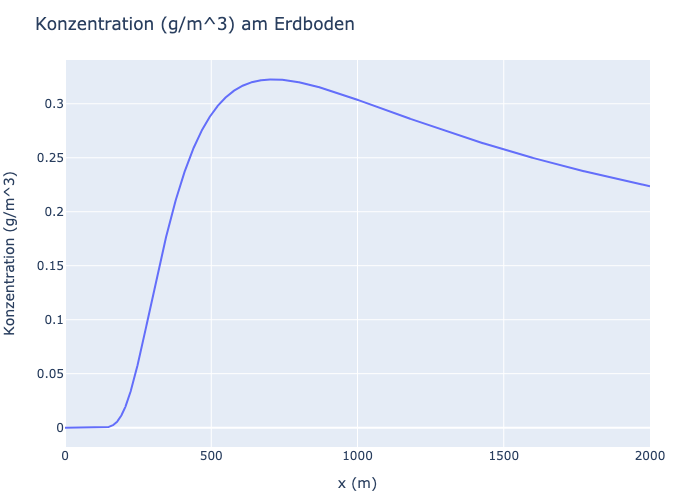
\includegraphics[scale=0.5]{Bilder/1b.png}
	\caption{Konzentrationsverteilung am Erdboden}
	\label{fig:my_label}
\end{figure}

Die maximale Konzentration wurde final rechnerisch mittels Julia bestimmt als
\begin{equation}
	c[0,711] = 0,32263  \frac{g}{m^3}
\end{equation}
\subsection{Aufgabenteil b}
Für den Vergleich zwischen Monte-Carlo-Modell und Gauß-Modell wurden beide Modelle in einem Contour-Plot visualisiert.  Für die optimale Visualisierung wurden verschiedene Partikelanzahlen visualisiert.
\begin{figure}[H]
	\centering
	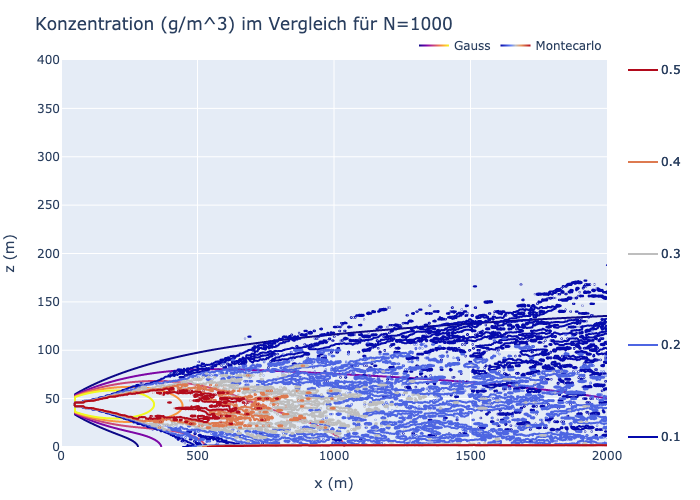
\includegraphics[scale=0.5]{Bilder/1b1k.png}
	\caption{Vergleich für N=1000}
	\label{fig:my_label}
\end{figure}
In Abb. 4 ist leider keine gute Annäherung des Montecarlo Modells an das Gaußmodell zu erkennen. Die Anzahl der Teilchen hat beim Montecarlo Modell einen hohen Einfluss auf die Güte des Modells. Bei einer geringeren Anzahl wie 

\begin{equation}
	N=1000
\end{equation}
sind extrem große Abweichungen zum Gaußmodell zu erkennen.
\begin{figure}[H]
	\centering
	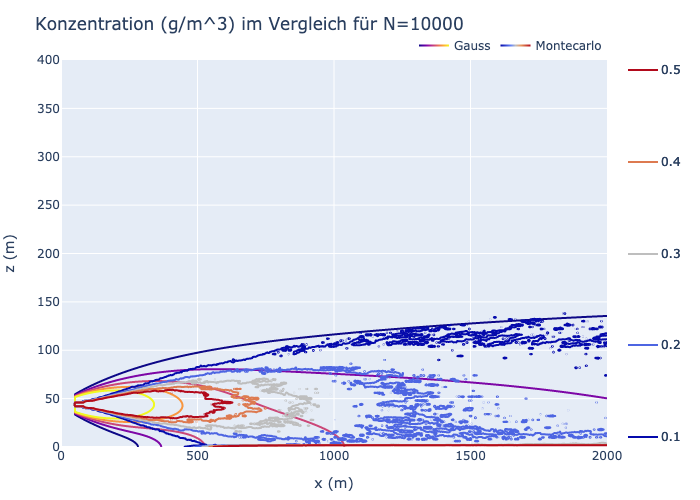
\includegraphics[scale=0.5]{Bilder/1b10k.png}
	\caption{Vergleich für N=10000}
	\label{fig:my_label}
\end{figure}
Bei einer mittleren Anzahl wie 

\begin{equation}
	N=10000
\end{equation}
gleicht sich das MC Modell bedeutend besser an das Gaußmodell an.
\begin{figure}[H]
	\centering
	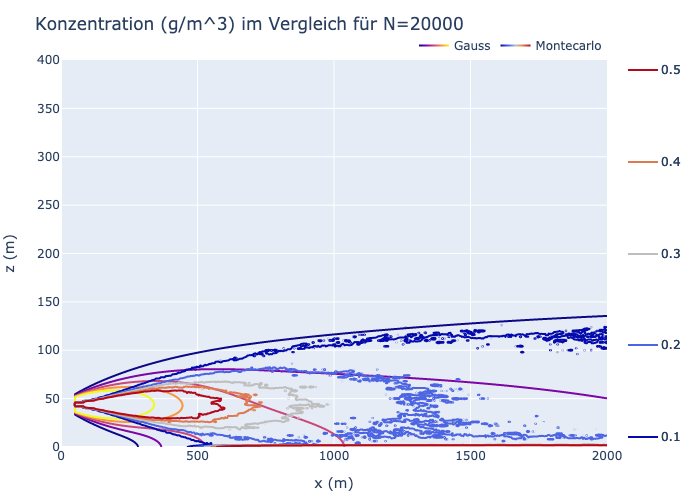
\includegraphics[scale=0.5]{Bilder/1b20k.png}
	\caption{Vergleich für N=20000}
	\label{fig:my_label}
\end{figure}
Bei einer hohen Anzahl wie 

\begin{equation}
	N=20000
\end{equation}
gleicht sich das MC Modell sehr gut an das Gaußmodell an.
\begin{figure}[H]
	\centering
	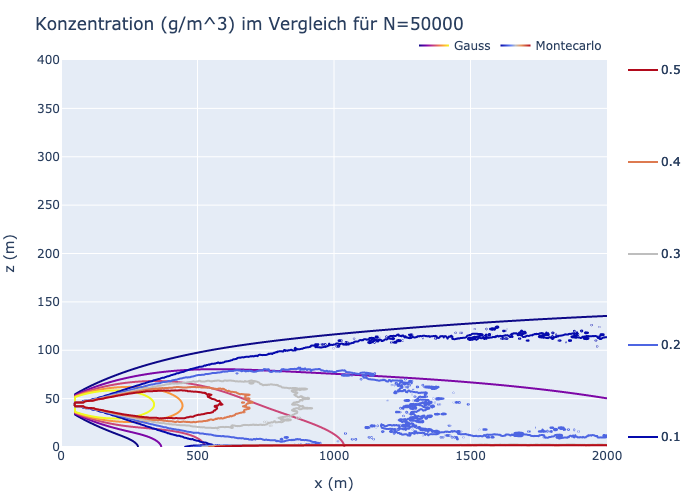
\includegraphics[scale=0.5]{Bilder/1b50k.png}
	\caption{Vergleich für N=50000}
	\label{fig:my_label}
\end{figure}
Abbildung 5  zeigt das mit meiner Hardware maximal mögliche Ergebnis. Jenseits von dieser Anzahl sind zwar noch leichte Verbesserungen zu erwarten, nichts destotrotz zeigt sich bei 

\begin{equation}
	N=50000
\end{equation}

eine extrem gute Annäherung an das Gauß-Modell. Für eine Ausreichende Statistik reichen aber bereits 
\begin{equation}
	N=20000
\end{equation}.
\section{Aufgabe 2}
In dieser Aufgabe sollte das Monte-Carlo-Modell mit der Prandtl-Schicht optimiert und die Ergebnisse durch das Prairie-Grass-Experiment validiert werden.
\begin{figure}[H]
	\centering
	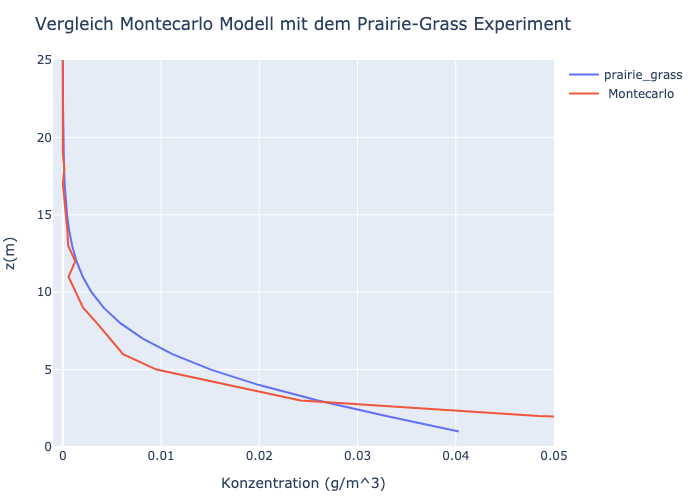
\includegraphics[scale=0.5]{Bilder/2back.png}
	\caption{Vergleich Prairie-Grass}
	\label{fig:my_label}
\end{figure}
\section{Aufgabe  3}
\subsection{Aufgabenteil a}
\begin{figure}[H]
	\centering
	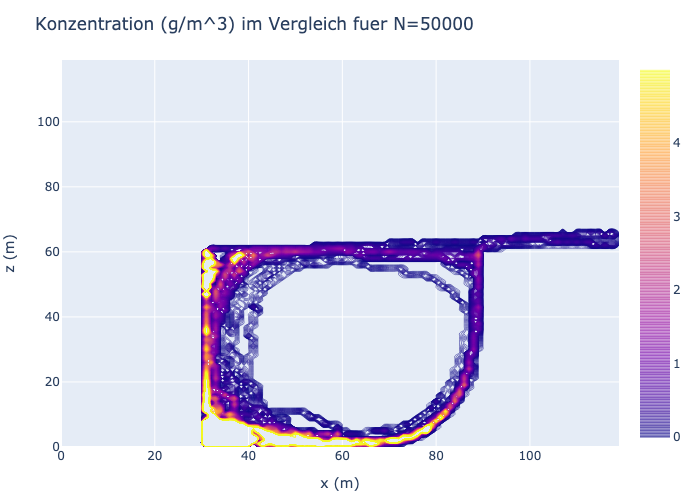
\includegraphics[scale=0.5]{Bilder/3k_xq=60.5.png}
	\caption{Konzentrationsverteilung am Erdboden}
	\label{fig:my_label}
\end{figure}

\subsection{Aufgabenteil b}

\begin{figure}[H]
	\centering
	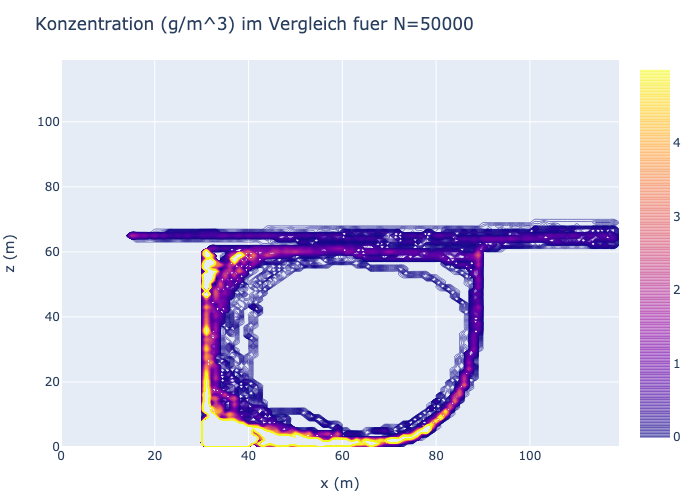
\includegraphics[scale=0.5]{Bilder/3k_xq=15.5.png}
	\caption{Konzentrationsverteilung am Erdboden}
	\label{fig:my_label}
\end{figure}
\section{Aufgabe  4}

\section{Quellcode}
\subsection{Aufgabe 2}
\lstinputlisting[language=Python]{Aufgabe2.jl}
\subsection{Aufgabe 3}
\lstinputlisting[language=Python]{Aufgabe3.jl}
\end{document}
